
    \chapter{Análise de requisitos de segurança}
    Neste capítulo, abordaremos todo o processo de desenvolvimento e análise de requisitos, desde a elicitação e definição dos requisitos de segurança, fundamentando-nos nos casos de uso indevido identificados em aplicações bancárias móveis, até a especificação e modelagem dos mesmos. 


    \section{Elicitação dos requisitos utilizando caso de uso indevido}

    A compreensão dos componentes chave de segurança em aplicações bancárias no Android é essencial para garantir a proteção dos dados dos usuários e a integridade das transações financeiras. A técnica de caso de uso indevido se destaca nesse contexto, pois permite modelar os cenários mais frequentes, citados na seção \ref{ameaças}, em que atores mal-intencionados tentam explorar fragilidades do sistema, fornecendo uma base sólida para a definição de requisitos de segurança.

    A técnica de caso de uso indevido, introduzida por \citeonline{Sindre2000}, complementa a elicitação tradicional de requisitos ao focar explicitamente em como um sistema pode ser comprometido. Ao invés de apenas definir como o sistema deve se comportar, os casos de uso indevido ilustram como o sistema pode ser atacado, permitindo a antecipação de ameaças específicas.
    
    Como vemos na figura \ref{misuses}, o diagrama inclui três principais atores: Usuário, Hacker, e Malware. O Usuário representa o cliente legítimo que utiliza a aplicação bancária para realizar ações como visualizar saldo, realizar login, validar transações, e executar transações financeiras. Cada uma dessas ações é modelada como um caso de uso, com várias camadas de segurança associadas, refletindo práticas recomendadas de segurança cibernética. Já o Hacker e o Malware representam as ameaças à segurança, como elas podem afetar uma aplicação bancária e como as medidas de prevenção são implementadas para mitigar esses riscos. Cada ameaça identificada está diretamente associada a casos de uso que envolvem interações críticas entre o usuário, o sistema e possíveis agentes maliciosos.

    \begin{figure}[H]
    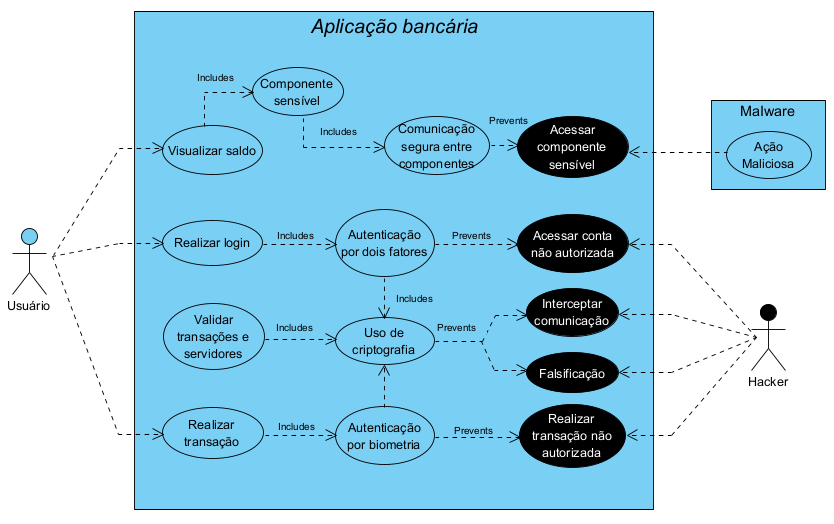
\includegraphics[width=17cm]{Imagens/misuse.png} 
    \caption{Casos de uso indevidos de aplicações bancárias}
    \label{misuses}
    \end{figure}
    
    Ao analisar essas ameaças, como malwares que visam roubo de credenciais e dados pessoais, fica clara a necessidade do desenvolvimento de requisitos que detalhem a implementação de mecanismos de segurança na comunicação entre processos na plataforma Android para proteção desses componentes sensíveis. 
    
    Similarmente, a identificação de vulnerabilidades em processos de autenticação deixa claro a importância da adoção de métodos de autenticação mais robustos, como autenticação multifator (MFA), biometria e pins numéricos, para mitigar riscos de acesso não autorizado.

    A criptografia, por sua vez, é fundamental para garantir a segurança dos dados em trânsito e em repouso. A análise dos casos de uso indevido encaminha a escolha de padrões criptográficos modernos que são capazes de resistir a ataques sofisticados, como AES-256-CBC, ECDSA e SHA-256. 
    
    Finalmente, a necessidade de proteger a comunicação entre o cliente e o servidor contra ataques de rede, como os ataques MITM, destaca diretamente a importância da adoção de protocolos de comunicação seguros, como o Transport Layer Security (TLS) 1.3.

    \section{Definição dos requisitos}
    Durante o processo de estudo, o objetivo foi encontrar um conjunto de pontos críticos e suas respectivas remediações de modo a entender as aplicações bancárias e por fim propor um modelo teórico capaz de tornar o ambiente seguro para o uso. A partir da análise do cenários de ameaças anterior, foi obtida uma base para a realização da definição dos requisitos de segurança necessários para mitigar esses riscos associados. Esses requisitos foram divididos em áreas como visto na figura \ref{visao}.

    \begin{figure}[H]
    \centering 
    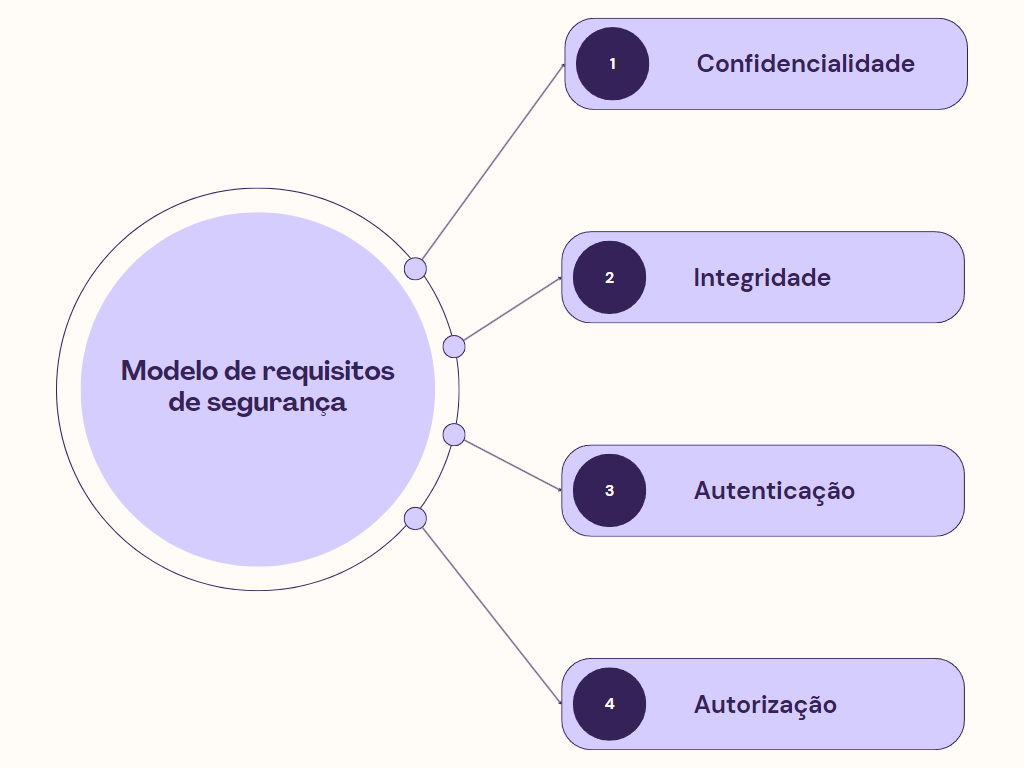
\includegraphics[width=10cm]{Imagens/arvre.png} 
    \caption{Visão geral dos requisitos de segurança}
    \label{visao}
    \end{figure}

    \begin{enumerate}

    \subsection{Requisitos de confidencialidade}

    \item O sistema deverá utilizar criptografia para armazenar senhas e chaves.
    
    \item A aplicação deverá utilizar TLS para realizar a comunicação com o servidor.
    
    \subsection{Requisitos de integridade}

    \item O sistema deverá armazenar o Hash de cada transação.

    \item O sistema deverá armazenar a assinatura digital do pagador em cada transação.

    \item O sistema deverá realizar a comunicação apenas com o servidor confiável.
    
    \subsection{Requisitos de autenticação}

    \item O acesso ao sistema deverá ser feito utilizando autenticação de multiplos fatores (MFA).

    \item O sistema deverá exigir Pin ou biometria para a realização de transações e pagamentos. 
    
    \subsection{Requisitos de autorização}

    \item O sistema não deve exportar componentes que não exigem interação externa. 

    \item O sistema deve exigir permissões para acessar os componentes exportados. 

    \item O sistema deve validar de intents recebidas nos componentes exportados. 

    \end{enumerate}


    \section{Especificação dos requisitos de segurança}
    A especificação dos requisitos de segurança é um processo crítico que envolve o definição clara, detalhada e estruturada dos requisitos de segurança definidos anteriormente. Na prática, ela atua como um guia detalhado para desenvolvedores, engenheiros de qualidade e outros stakeholders, assegurando que todos tenham uma compreensão comum do que deve ser construído e como o sistema deve operar. Ela serve como uma ponte entre a análise de requisitos, onde as necessidades dos usuários e as restrições do sistema são identificadas, e a fase de desenvolvimento, onde essas necessidades são implementadas.
    
    \begin{enumerate}
    
        \subsection{Requisitos de Confidencialidade}
    
        \item \textbf{O sistema deverá utilizar criptografia para armazenar senhas e chaves}
        \begin{enumerate}
            \item[1.1] Identificar os dados que requerem criptografia.
            \item[1.2] Configurar o sistema para usar o algoritmo de criptografia Advanced Encryption Standard com uma chave de 256 bits no modo Cipher Block Chaining (AES-256-CBC) para senhas e chaves.
            \item[1.3] Gerar e armazenar chaves criptográficas de forma segura utilizando o Android KeyStore.
            \item[1.4] Utilizar os algoritmos para criptografar as senhas e chaves.
            \item[1.5] Armazenar o conteúdo criptografado no banco de dados.
            \item[1.6] Encerrar a sessão de criptografia e liberar os recursos de criptografia.
        \end{enumerate}
        
        \item \textbf{O sistema deverá utilizar TLS para realizar a comunicação}
        \begin{enumerate}
            \item[2.1] Configurar o sistema para estabelecer conexões seguras utilizando TLS 1.2 ou superior.
            \item[2.2] Iniciar a comunicação entre cliente e servidor.
            \item[2.3] Setar os parâmetros criptográficos do TLS com o servidor.
            \item[2.4] Verificar a validade do certificado digital do servidor.
            \item[2.5] Estabelecer a conexão TLS após a validação do certificado.
            \item[2.6] Transmitir dados de forma segura utilizando o canal TLS.
            \item[2.7] Encerrar a conexão TLS após a conclusão da comunicação.
        \end{enumerate}
    
        \subsection{Requisitos de Integridade}
    
        \item \textbf{O sistema deverá armazenar o Hash de cada transação}
        \begin{enumerate}
            \item[3.1] Gerar um hash criptográfico para cada transação utilizando o algoritmo Secure Hash Algorithm com valor hash de 256 bits (SHA-256).
            \item[3.2] Associar o hash à transação correspondente.
            \item[3.3] Verificar o hash ao acessar ou modificar a transação.
            \item[3.4] Armazenar o hash de forma segura no banco de dados.
            \item[3.5] Auditar periodicamente os hashes armazenados para garantir integridade.
            \item[3.6] Validar a consistência do hash durante o processamento das transações.
            \item[3.7] Registrar o resultado da validação de hash para auditoria futura.
        \end{enumerate}
    
        \item \textbf{O sistema deverá armazenar a assinatura digital do pagador em cada transação}
        \begin{enumerate}
            \item[4.1] Capturar a assinatura digital do pagador, feita com o algoritmo Elliptic Curve Digital Signature Algorithm (ECDSA), no momento da transação.
            \item[4.2] Validar a assinatura digital para garantir sua autenticidade.
            \item[4.3] Associar a assinatura digital à transação correspondente.
            \item[4.4] Armazenar a assinatura digital de forma segura no banco de dados.
            \item[4.5] Verificar a assinatura digital antes de processar a transação.
            \item[4.6] Auditar as assinaturas digitais armazenadas regularmente.
            \item[4.7] Registrar o status de verificação da assinatura digital para referência futura.
        \end{enumerate}
    
        \item \textbf{O sistema deverá realizar a comunicação apenas com o servidor confiável}
        \begin{enumerate}
            \item[5.1] Armazenar no código fonte da aplicação o certificado digital dos servidores confiáveis.
            \item[5.2] Configurar o cliente para usar exclusivamente os certificados digitais armazenados para comunicação.
            \item[5.3] Validar esses certificados digitais ao estabelecer uma conexão com o servidor.
            \item[5.4] Rejeitar conexões com servidores que não utilizem um dos certificados armazenados.
            \item[5.5] Registrar tentativas de conexão não autorizadas para análise de segurança.
        \end{enumerate}
    
        \subsection{Requisitos de Autenticação}
    
        \item \textbf{O acesso ao sistema deverá ser feito utilizando autenticação de multiplos fatores (MFA)}
        \begin{enumerate}
            \item[6.1] Exibir a interface de login para o usuário.
            \item[6.2] Solicitar nome de usuário e senha.
            \item[6.3] Verificar usuário e senha cadastrada.
            \item[6.4] Enviar senha de uso único baseada em tempo ao número cadastrado por SMS.
            \item[6.5] Solicitar a senha de uso.
            \item[6.6] Verificar senha.
            \item[6.7] Liberar o acesso ao perfil de usuário  após a validação dos dois fatores bem-sucedida.
            \item[6.8] Permitir acesso às funcionalidades do sistema.
            \item[6.9] Finalizar processo.
        \end{enumerate}
    
        \item \textbf{O sistema deverá exigir Pin ou biometria para a realização de transações e pagamentos}
        \begin{enumerate}
            \item[7.1] Solicitar Pin ou autenticação biométrica ao iniciar uma transação.
            \item[7.2] Verificar o Pin ou a biometria fornecida pelo usuário.
            \item[7.3] Validar a autenticidade do usuário antes de processar a transação.
            \item[7.4] Processar a transação ou pagamento após a validação bem-sucedida.
            \item[7.5] Registrar as transações realizadas para auditoria e análise de segurança.
            \item[7.6] Encerrar o processo de transação após confirmação e notificar o usuário.
        \end{enumerate}
    
        \subsection{Requisitos de Autorização}
    
        \item \textbf{O sistema não deve exportar componentes que não têm interação externa}
        \begin{enumerate}
            \item[8.1] Identificar componentes que não necessitam de interação externa.
            \item[8.2] Definir como ``false'' a exportação desses componentes.
            \item[8.3] Verificar a configuração de componentes para garantir que não estão exportados indevidamente.
            \item[8.4] Monitorar o sistema para identificar tentativas de acesso a componentes não exportados.
            \item[8.5] Registrar qualquer tentativa de interação não autorizada para auditoria.
            \item[8.6] Encerrar processos que tentem acessar componentes não exportados.
        \end{enumerate}
    
        \item \textbf{O sistema deve exigir permissões para acessar os componentes exportados}
        \begin{enumerate}
            \item[9.1] Identificar os componentes exportados da aplicação.
            \item[9.2] Definir o parâmetro protectionLevel como ``signature'' nesses componentes.
            \item[9.3] Definir o parâmetro permission como ``READ\_PROVIDER'' nos provedores de conteúdo.
            \item[9.4] Monitorar o sistema para identificar tentativas de acesso não autorizadas a esses componentes.
            \item[9.5] Registrar qualquer tentativa de interação não autorizada para auditoria.
            \item[9.6] Encerrar processos que tentem acessar componentes sem autorização.
        \end{enumerate}
    
        \item \textbf{O sistema deve validar intents recebidas nos componentes exportados}
        \begin{enumerate}
            \item[10.1] Capturar intents recebidas nos componentes exportados.
            \item[10.2] Verificar a autenticidade e a origem das intents recebidas.
            \item[10.3] Validar os dados contidos nas intents antes de processá-las.
            \item[10.4] Processar a intent se for validada com sucesso.
            \item[10.5] Registrar todas as intents recebidas para auditoria e análise de segurança.
            \item[10.6] Monitorar o comportamento dos componentes exportados para detectar intents suspeitas.
            \item[10.7] Encerrar o processamento de intents inválidas ou não autorizadas.
        \end{enumerate}
    
    \end{enumerate}

    
    \section{Modelagem de dados e processos}
    A modelagem de dados e processos é uma fase essencial no desenvolvimento de sistemas, servindo como a base para a construção de soluções tecnológicas que sejam eficientes, escaláveis e alinhadas com os objetivos organizacionais. Este processo envolve a representação estruturada das informações que o sistema irá manipular (modelagem de dados) e a definição dos fluxos de trabalho e das atividades que o sistema deve executar (modelagem de processos).
    
    Dessa forma, exploraremos os princípios e técnicas de modelagem de dados e processos, demonstrando como os requisitos de segurança se relacionam com o sistema e suas funcionalidades.
    
    \subsection{Diagramas UML}

    O diagrama de classe, visto na figura \ref{cript} representa a classe Cliente e seus atributos e métodos. A classe possui os atributos senha, que é uma informação considerada sensível no processo de armazenamento. Este diagrama sugere que os dados sensíveis, no caso a senha, seja criptografado dentro de um sistema bancário.

    \begin{figure}[H]
    \centering 
    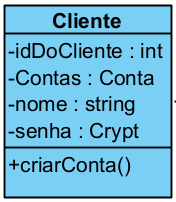
\includegraphics[width=6cm]{Imagens/cript.png} 
    \caption{Informações armazenadas em texto cifrado}
    \label{cript}
    \end{figure}

    O diagrama de sequência, observado na figura \ref{tls}, mostra o fluxo de interação entre a aplicação bancária e o servidor durante o processo da realização de uma comunicação criptografada, utilizando o TLS. A aplicação bancária envia uma lista de cifras com o conjunto de algoritmos que eles podem utilizar para a comunicação. Este conjunto tem vários parâmetros, sendo o primeiro o método de troca de chaves, o segundo o método de autenticação, terceiro o algoritmo simétrico com seu tamanho de chave e operação e por último o algoritmo de hash utilizado. Com isso, o servidor retorna a cifra escolhida, um certificado com uma assinatura digital e a server key exchange, que são os parâmetros utilizados para gerar a chave de criptografia. Dessa forma, a aplicação e o servidor conseguem realizar a comunicação criptografadas e segura.

    \begin{figure}[H]
    \centering 
    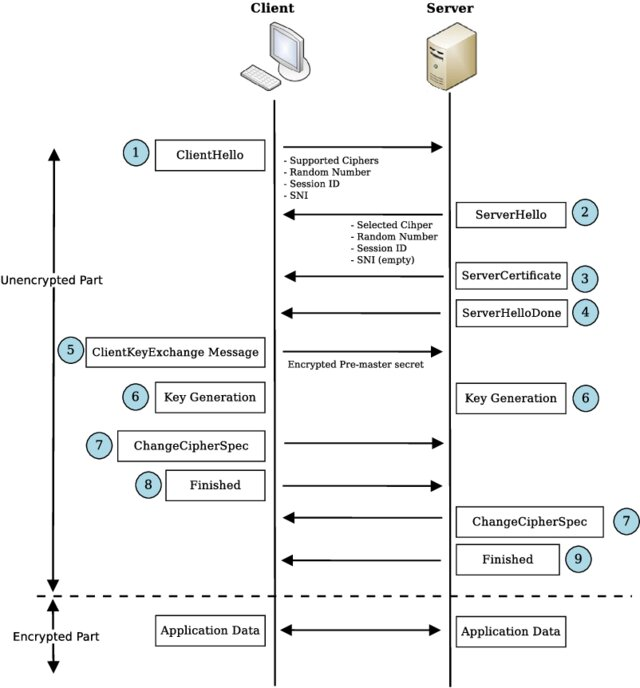
\includegraphics[width=13cm]{Imagens/tlshandshake.jpg} 
    \caption{Funcionamento do protocolo TLS}
    \label{tls}
    \cite{tls2016}
    \end{figure}

    O diagrama de classe, visto na figura \ref{transacao} representa a classe Transação e seus atributos e métodos. A classe possui os atributos verifIntegridade (responsável pela verificação de integridade de uma transação) e assinaturaDigital (Responsável pelo não repúdio e autenticidade da transação), utilizados para verificar a integridade e autenticidade dos dados. Este diagrama garante que os dados não foram alterados ou danificados dentro de um sistema bancário.
    
    \begin{figure}[H]
    \centering 
    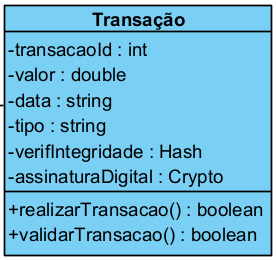
\includegraphics[width=6cm]{Imagens/integridade.png} 
    \caption{Armazenamento de Hash e Assinatura digital}
    \label{transacao}
    \end{figure}    

    O diagrama de sequência, observado na figura \ref{totp}, mostra o fluxo de interação entre um usuário, a aplicação bancária, o servidor e o banco de dados durante o processo de login. O usuário solicita o login e envia suas credenciais pré cadastradas. O servidor valida as credenciais consultando o banco de dados e, após a validação, solicita uma autenticação multifator (MFA). O usuário envia o MFA, que é validado, e uma sessão segura é gerada, resultando em um login bem-sucedido. 
    
    \begin{figure}[H]
    \centering 
    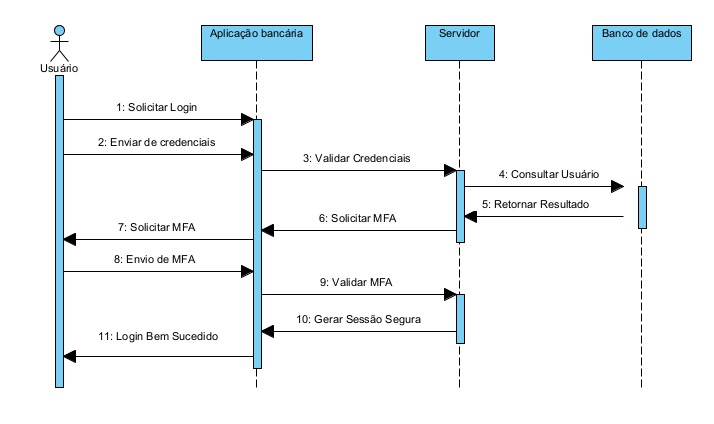
\includegraphics[width=15cm]{Imagens/login.png} 
    \caption{Autenticação multifatorial utilizando Login, Senha e TOTP}
    \label{totp}
    \end{figure}

    O diagrama de sequência, ilustrado na figura \ref{pin}, detalha o processo de solicitação e aprovação de uma transação ou pagamento. O usuário inicia a solicitação e envia um PIN para a aplicação bancária, que então o repassa ao servidor. O servidor valida os dados, verifica a integridade da transação e registra a operação no banco de dados. Após o registro, o servidor retorna o resultado, e a transação é aprovada. Este fluxo assegura que cada etapa seja validada e registrada adequadamente antes de concluir a transação.

    \begin{figure}[H]
    \centering 
    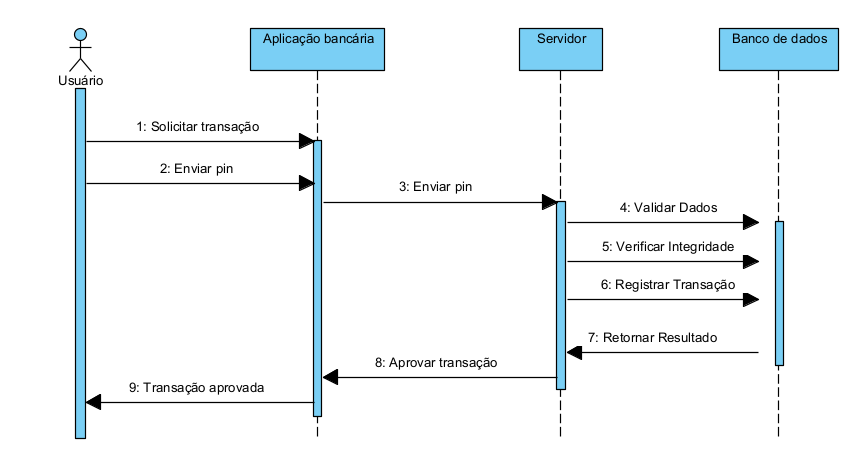
\includegraphics[width=15cm]{Imagens/pagamento.png} 
    \caption{Autenticação por Pin}
    \label{pin}
    \end{figure}

    O diagrama de caso de uso indevido, observado na figura \ref{malware}, ilustra a proteção de componentes sensíveis, exportados e consentidos em uma aplicação bancária contra ações maliciosas de malware. Para evitar ataques, são implementados controles como desabilitar a exportação de componentes (Exported:"false"), aplicar níveis de proteção (ProtectionLevel), e sanitarizar intents (IntentSanitizer). Esses mecanismos ajudam a mitigar as ações maliciosas que tentam explorar vulnerabilidades na aplicação.

    \begin{figure}[H]
    \centering 
    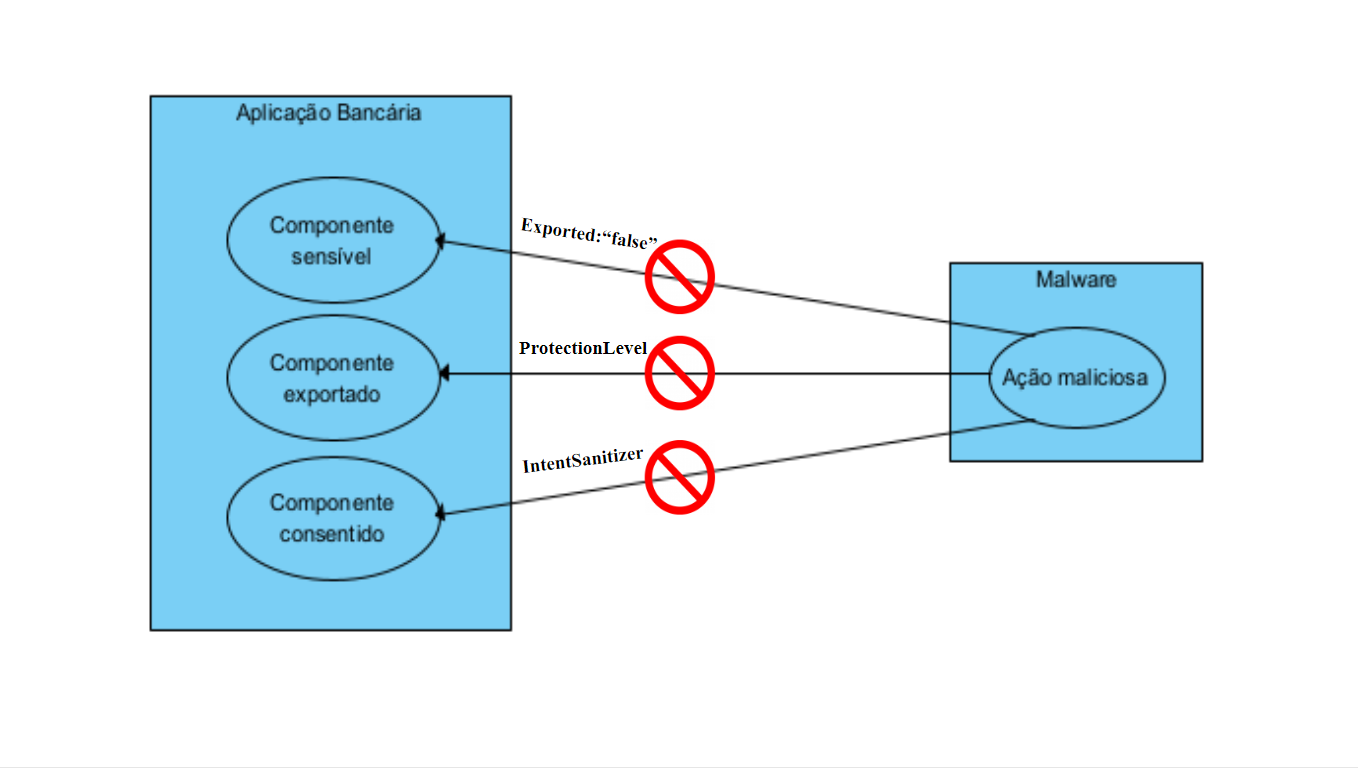
\includegraphics[width=14cm]{Imagens/malware.png} 
    \caption{Caso de uso indevido: ataque malware}
    \label{malware}
    \end{figure}
    